\documentclass[11pt,letterpaper]{article}
\usepackage{acl2015}
\usepackage{times}
\usepackage{latexsym}
% \setlength\titlebox{5cm}    % Expanding the titlebox

%%% Custom additions %%%
\usepackage{url}
\usepackage[leqno, fleqn]{amsmath}
\usepackage{amssymb}
\usepackage{qtree}
\usepackage{graphicx}
\usepackage{booktabs}
\usepackage{multirow}
\usepackage{colortbl}
\usepackage{caption}
\usepackage{subcaption}
\usepackage{color}
\usepackage{xcolor}
\usepackage{tikz}
\usepackage{ifthen}
\usepackage{framed}

\newcount\colveccount
\newcommand*\colvec[1]{
        \global\colveccount#1
        \begin{bmatrix}
        \colvecnext
}
\def\colvecnext#1{
        #1
        \global\advance\colveccount-1
        \ifnum\colveccount>0
                \\
                \expandafter\colvecnext
        \else
                \end{bmatrix}
        \fi
}

\newcommand{\nateq}{\equiv}
\newcommand{\natind}{\mathbin{\#}}
\newcommand{\natneg}{\mathbin{^{\wedge}}}
\newcommand{\natfor}{\sqsubset}
\newcommand{\natrev}{\sqsupset}
\newcommand{\natalt}{\mathbin{|}}
\newcommand{\natcov}{\mathbin{\smallsmile}}

\newcommand{\plneg}{\mathop{\textit{not}}}
\newcommand{\pland}{\mathbin{\textit{and}}}
\newcommand{\plor}{\mathbin{\textit{or}}}

\newcommand{\shift}{\textsc{shift}}
\newcommand{\reduce}{\textsc{reduce}}

% Strikeout
\newlength{\howlong}\newcommand{\strikeout}[1]{\settowidth{\howlong}{#1}#1\unitlength0.5ex%
\begin{picture}(0,0)\put(0,1){\line(-1,0){\howlong\divide\unitlength}}\end{picture}}

\newcommand{\True}{\texttt{T}}
\newcommand{\False}{\texttt{F}}
\usepackage{stmaryrd}
\newcommand{\sem}[1]{\ensuremath{\llbracket#1\rrbracket}}

\newcommand{\mynote}[1]{{\color{blue}#1}}
\newcommand{\tbchecked}[1]{{\color{red}#1}}

\usepackage{gb4e}
\noautomath
 
\def\ii#1{\textit{#1}}
\newcommand{\word}[1]{\emph{#1}}
\newcommand{\fulllabel}[2]{\b{#1}\newline\textsc{#2}}

%%%%%%%%%%%%%%%%%%%%%%%%%%%%%%%%%%%%%%%%%%%%%%%%%%%%%%%%%%%%%%%%%%%%%%
%%%%% Code to simulate natbib's citealt, which prints citations with
%%%%% no parentheses:

\makeatletter
\def\citealt{\def\citename##1{{\frenchspacing##1} }\@internalcitec}
\def\@citexc[#1]#2{\if@filesw\immediate\write\@auxout{\string\citation{#2}}\fi
  \def\@citea{}\@citealt{\@for\@citeb:=#2\do
    {\@citea\def\@citea{;\penalty\@m\ }\@ifundefined
       {b@\@citeb}{{\bf ?}\@warning
       {Citation `\@citeb' on page \thepage \space undefined}}%
{\csname b@\@citeb\endcsname}}}{#1}}
\def\@internalcitec{\@ifnextchar [{\@tempswatrue\@citexc}{\@tempswafalse\@citexc[]}}
\def\@citealt#1#2{{#1\if@tempswa, #2\fi}}
\makeatother

%%%%%%%%%%%%%%%%%%%%%%%%%%%%%%%%%%%%%%%%%%%%%%%%%%%%%%%%%%%%%%%%%%%%%%


%%% %%%

\title{NSHRDLU?}

\author{
Samuel R.\ Bowman$^{\ast\dag}$ \\
\texttt{sbowman@stanford.edu} \\
\And
Jon Gauthier$^{\dag\ddag}$ \\
\texttt{angeli@stanford.edu} \\
\AND
Christopher Potts$^{\ast}$\\
\texttt{cgpotts@stanford.edu}
\And
Christopher D.\ Manning$^{\ast\dag\S}$\\
\texttt{manning@stanford.edu}\\
\AND\\[-3ex]
{$^{\ast}$Stanford Linguistics\quad
$^{\dag}$Stanford NLP Group}\\
{$^{\ddag}$Stanford Symbolic Systems\quad
$^{\S}$Stanford Computer Science}
}

\date{}

\makeatletter
\newcommand{\@BIBLABEL}{\@emptybiblabel}
\newcommand{\@emptybiblabel}[1]{}
\definecolor{black}{rgb}{0,0,0}
\makeatother
\usepackage[breaklinks, colorlinks, linkcolor=black, urlcolor=black, citecolor=black]{hyperref}

\def\t#1{#1}
\def\b#1{\t{\textbf{#1}}}
\def\colspaceS{2.25mm}
\def\colspaceM{4.0mm}
\def\colspaceL{4.25mm}

\newcommand\todo[1]{\textcolor{blue}{\textbf{TODO:} #1}}

\begin{document}
\maketitle

This project aims to build neural network models that can jointly learn to parse sentences and to use those parses to guide semantic composition.

Table~\ref{models-table} shows the sequence of model designs that we plan to build. 


\begin{table*}[t]
  \centering\small
  \begin{tabular}{ccccc} 
    \toprule
    Name & Stack Representation & Input Representation & Ops Classifier & Op Predictions Used in Training \\ 
    \midrule
Model 0 & Discrete & Op. sequence & N & -- \\
Model 1 & Discrete & \bf Discrete Buffer & \bf Y: Directly supervised & \bf N \\
Model 2 & Discrete & Discrete Buffer & Y: Directly supervised & \bf Y \\
Model 3 & \bf Soft & \bf Soft Buffer & Y: Directly supervised & Y \\
Model 4 & Soft & Soft Buffer & \bf Y: Indirectly supervised & Y \\
    \bottomrule
  \end{tabular}
  \protect\caption{\protect\label{models-table}Model variants, ordered by increasing reliance on learning. Bolding indicates the differences between each model and its parent model.} 
\end{table*}

\section{Models}

\subsection{Model 0}

Model 0 in its simplest form computes the same function as a plain TreeRNN, but uses a stack and a recurrent input reader instead of a tree as its graph structure. \todo{Model 0 figure.} We expect it to be substantially faster than conventional TreeRNN implementations, since it readily supports batched matrix--vector multiplications, allowing it to fast CPU libraries and to function well on GPUs.

\subsection{Model 1}

%!TEX root = hard_stack_paper/paper.tex

\begin{figure*}[t]
\begin{subfigure}[t]{\textwidth}
\centering
\scalebox{0.72}{%
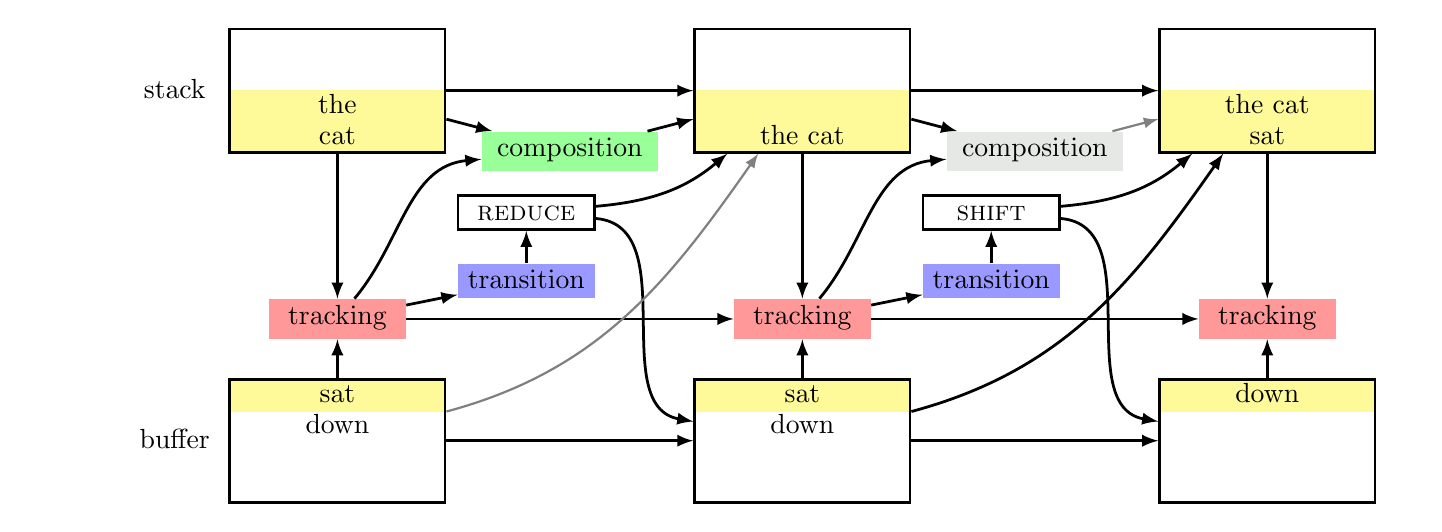
\begin{tikzpicture}
    \def\dx{21pt}
    \def\dy{11pt}
    \def\sy{12*\dy}
    \def\oxb{8*\dx}
    \def\by{0pt}
    \def\ox{0*\oxb}

    \tikzstyle{label}=[text width=35mm,align=center,text height=2mm]    
    \tikzstyle{word}=[text width=35mm,align=center,text height=2mm]    
    \tikzstyle{tracker}=[fill=red!40,text width=15mm,align=center,text height=2mm]
    \tikzstyle{softmax}=[fill=blue!40,text width=15mm,align=center,text height=2mm]
    \tikzstyle{comp}=[fill=green!40,text width=20mm,align=center,text height=2mm]
    \tikzstyle{compoff}=[fill=green!10!black!10,text width=20mm,align=center,text height=2mm]
    \tikzstyle{result}=[line width=1pt,draw=black,text width=15mm,align=center,text height=2mm]    
    \tikzstyle{sbox}=[line width=1pt,draw=black,text width=25mm,align=center,text height=13.3mm]
    \tikzstyle{bbox}=[line width=1pt,draw=black,text width=25mm,align=center,text height=13.3mm]
    \tikzstyle{focus1}=[fill=yellow!40,text width=25mm,align=center,text height=2mm]
    \tikzstyle{focus2}=[fill=yellow!40,text width=25mm,align=center,text height=5.5mm]

    \node[label]  (sl) at (\ox-0.35*\oxb+0*\dx,\by+1*\dy) {buffer};

    \node[focus1] (0bb) at  (\ox+0*\dx,2.5*\dy) {};
    \node[word]  (0b3) at (\ox+0*\dx,\by-0.5*\dy) {};
    \node[word]  (0b2) at (\ox+0*\dx,\by+1.5*\dy) {down};
    \node[word]  (0b1) at (\ox+0*\dx,\by+2.5*\dy) {sat};
    \node[bbox] (0bb) at  (\ox+0*\dx,\by+1.0*\dy) {};
    
    \node[label]  (sl) at (\ox-0.35*\oxb+0*\dx,\sy+0.5*\dy) {stack};
    
    \node[focus2] (0sb) at  (\ox+0*\dx,\sy-0.5*\dy) {};
    \node[word]  (0s1) at (\ox+0*\dx,\sy-1*\dy) {cat};
    \node[word]  (0s2) at (\ox+0*\dx,\sy+0*\dy) {the};
    \node[word]  (0s3) at (\ox+0*\dx,\sy+1*\dy) {};
    \node[sbox] (0sb) at  (\ox+0*\dx,\sy+0.5*\dy) {};
    
    \node[comp] (0c) at  (\ox+0.5*\oxb,\sy-1.5*\dy) {composition};
    
    \node[tracker] (0t) at  (\ox+0*\dx,5*\dy) {tracking};
    \node[softmax] (0sm) at  (\ox+3.25*\dx,6.25*\dy) {transition};
    \node[result] (0so) at  (\ox+3.25*\dx,8.5*\dy) {\reduce};
    
    \def\ox{1*\oxb}

    \node[focus1] (1bb) at  (\ox+0*\dx,2.5*\dy) {};
    \node[word]  (1b3) at (\ox+0*\dx,\by-0.5*\dy) {};
    \node[word]  (1b2) at (\ox+0*\dx,\by+1.5*\dy) {down};
    \node[word]  (1b1) at (\ox+0*\dx,\by+2.5*\dy) {sat};
    \node[bbox] (1bb) at  (\ox+0*\dx,\by+1*\dy) {};
    
    \node[focus2] (1sb) at  (\ox+0*\dx,\sy-0.5*\dy) {};
    \node[word]  (1s1) at (\ox+0*\dx,\sy-1*\dy) {the cat};
    \node[word]  (1s2) at (\ox+0*\dx,\sy+0*\dy) {};
    \node[word]  (1s3) at (\ox+0*\dx,\sy+1*\dy) {};
    \node[sbox] (1sb) at  (\ox+0*\dx,\sy+0.5*\dy) {};
    
    \node[compoff] (1c) at  (\ox+0.5*\oxb,\sy-1.5*\dy) {composition};
    
    \node[tracker] (1t) at  (\ox+0*\dx,5*\dy) {tracking};
    \node[softmax] (1sm) at  (\ox+3.25*\dx,6.25*\dy) {transition};
    \node[result] (1so) at  (\ox+3.25*\dx,8.5*\dy) {\shift};
     
    \def\ox{2*\oxb}

    \node[focus1] (2bb) at  (\ox+0*\dx,2.5*\dy) {};
    \node[word]  (2b3) at (\ox+0*\dx,\by-0.5*\dy) {};
    \node[word]  (2b2) at (\ox+0*\dx,\by+1.5*\dy) {};
    \node[word]  (2b1) at (\ox+0*\dx,\by+2.5*\dy) {down};
    \node[bbox] (2bb) at  (\ox+0*\dx,\by+1*\dy) {};
    
    \node[focus2] (2sb) at  (\ox+0*\dx,\sy-0.5*\dy) {};
    \node[word]  (2s1) at (\ox+0*\dx,\sy-1*\dy) {sat};
    \node[word]  (2s2) at (\ox+0*\dx,\sy+0*\dy) {the cat};
    \node[word]  (2s3) at (\ox+0*\dx,\sy+1*\dy) {};
    \node[sbox] (2sb) at  (\ox+0*\dx,\sy+0.5*\dy) {};
   
    \node[tracker] (2t) at  (\ox+0*\dx,5*\dy) {tracking};

    
    \pgfsetarrowsend{latex}
    \tikzstyle{fwd} = [draw=black, line width=1pt]
    \tikzstyle{gated} = [draw=black!50, line width=0.8pt]

    \draw [fwd] (0sb) -- (0t);
    \draw [fwd] (0bb) -- (0t);
    \draw [fwd] (0t) -- (0sm);
    \draw [fwd] (0sm) -- (0so);
    \draw [fwd] (0sb) -- (0c);
    
    \draw [fwd] (0t) -- (1t);
    \draw [fwd] (0t) to[out=50,in=-175] (0c);
    \draw [fwd] (0sb) -- (1sb);
    \draw [fwd] (0bb) -- (1bb);
    \draw [fwd] (0so) to[out=5,in=-140] (1sb);
    \draw [fwd] (0so) to[out=-5,in=170] (1bb);
    \draw [gated] (0bb) to[out=15,in=-125] (1sb);
    \draw [fwd] (0c) -- (1sb);

    \draw [fwd] (1sb) -- (1t);
    \draw [fwd] (1bb) -- (1t);
    \draw [fwd] (1t) -- (1sm);
    \draw [fwd] (1sm) -- (1so);
    \draw [fwd] (1sb) -- (1c);
    
    \draw [fwd] (1t) -- (2t);
    \draw [fwd] (1t) to[out=50,in=-175] (1c);
    \draw [fwd] (1sb) -- (2sb);
    \draw [fwd] (1bb) -- (2bb);
    \draw [fwd] (1so) to[out=5,in=-140] (2sb);
    \draw [fwd] (1so) to[out=-5,in=170] (2bb);
    \draw [fwd] (1bb) to[out=15,in=-125] (2sb);
    \draw [gated] (1c) -- (2sb);

    \draw [fwd] (2sb) -- (2t);
    \draw [fwd] (2bb) -- (2t);


  \end{tikzpicture}}
  
 \caption{The SPINN model unrolled for two transitions during the processing of the sentence \word{the cat sat down}. `Tracking', `transition', and `composition' are neural network layers. Gray arrows indicate connections which are blocked by a gating function.}\label{fig:model:1d}
  
\end{subfigure}\\\\\\
\begin{subfigure}[t]{\textwidth}
\centering
\scalebox{0.49}{%
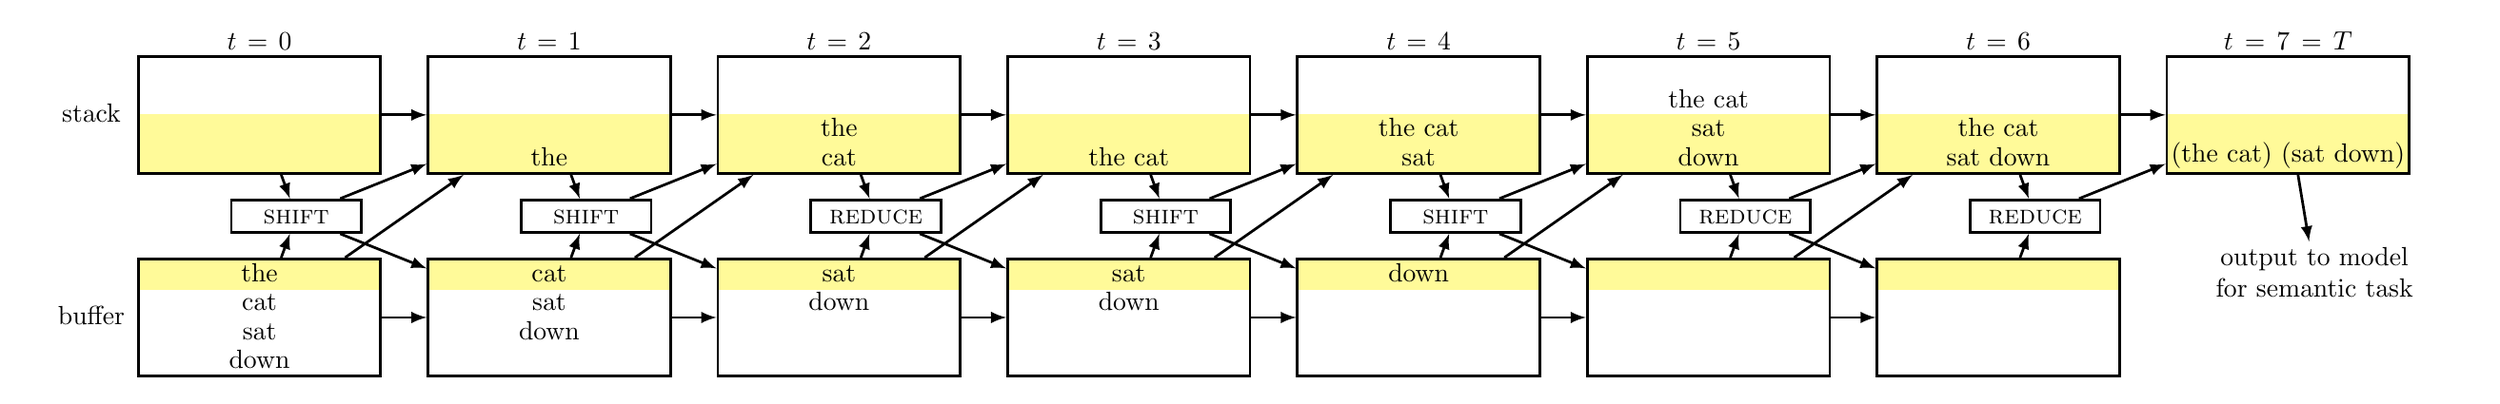
\begin{tikzpicture}
    \def\dx{20pt}
    \def\dy{11pt}
    \def\sy{7*\dy}
    \def\oxb{5.5*\dx}
    \def\by{0pt}
    \def\oxs{0pt}

    \tikzstyle{label}=[text width=15mm,align=center,text height=2mm]    
    \tikzstyle{word}=[text width=32mm,align=center,text height=2mm]    
    \tikzstyle{tracker}=[fill=red!40,text width=15mm,align=center,text height=2mm]
    \tikzstyle{softmax}=[text width=40mm,align=center,text height=2mm]
    \tikzstyle{comp}=[fill=green!40,text width=20mm,align=center,text height=2mm]
    \tikzstyle{result}=[line width=1pt,draw=black,text width=15mm,align=center,text height=2mm]    
    \tikzstyle{sbox}=[line width=1pt,draw=black,text width=30mm,align=center,text height=13.3mm]
    \tikzstyle{bbox}=[line width=1pt,draw=black,text width=30mm,align=center,text height=13.3mm]
    \tikzstyle{focus1}=[fill=yellow!40,text width=30mm,align=center,text height=2mm]
    \tikzstyle{focus2}=[fill=yellow!40,text width=30mm,align=center,text height=5.5mm]

    \def\ox{0*\oxb+\oxs}
    
    \node[label]  (sl) at (\ox-0.58*\oxb+0*\dx,\by+0.5*\dy) {buffer};
    
    \node[label]  (sl) at (\ox-0.58*\oxb+0*\dx,\sy+0.5*\dy) {stack};

    \node[label]  (00l) at (\ox+0*\dx,\sy+3*\dy) {$t=0$};

    \node[focus1] (00bb) at  (\ox+0*\dx,2*\dy) {};
    \node[word]  (00b3) at (\ox+0*\dx,\by-1*\dy) {down};
    \node[word]  (00b2) at (\ox+0*\dx,\by+0*\dy) {sat};
    \node[word]  (00b1) at (\ox+0*\dx,\by+1*\dy) {cat};
    \node[word]  (00b1) at (\ox+0*\dx,\by+2*\dy) {the};
    \node[bbox] (00bb) at  (\ox+0*\dx,\by+0.5*\dy) {};
        
    \node[focus2] (00sb) at  (\ox+0*\dx,\sy-0.5*\dy) {};
    \node[word]  (00s1) at (\ox+0*\dx,\sy-1*\dy) {};
    \node[word]  (00s2) at (\ox+0*\dx,\sy+0*\dy) {};
    \node[word]  (00s3) at (\ox+0*\dx,\sy+1*\dy) {};
    \node[sbox] (00sb) at  (\ox+0*\dx,\sy+0.5*\dy) {};
    
    \node[result] (00so) at  (\ox+0.7*\dx,4*\dy) {\shift};
              
    \def\ox{1*\oxb+\oxs}

    \node[label]  (0l) at (\ox+0*\dx,\sy+3*\dy) {$t=1$};

    \node[focus1] (0bb) at  (\ox+0*\dx,2*\dy) {};
    \node[word]  (00b3) at (\ox+0*\dx,\by-1*\dy) {};
    \node[word]  (00b2) at (\ox+0*\dx,\by+0*\dy) {down};
    \node[word]  (00b1) at (\ox+0*\dx,\by+1*\dy) {sat};
    \node[word]  (00b1) at (\ox+0*\dx,\by+2*\dy) {cat};
    \node[bbox] (0bb) at  (\ox+0*\dx,\by+0.5*\dy) {};
        
    \node[focus2] (0sb) at  (\ox+0*\dx,\sy-0.5*\dy) {};
    \node[word]  (0s1) at (\ox+0*\dx,\sy-1*\dy) {the};
    \node[word]  (0s2) at (\ox+0*\dx,\sy+0*\dy) {};
    \node[word]  (0s3) at (\ox+0*\dx,\sy+1*\dy) {};
    \node[sbox] (0sb) at  (\ox+0*\dx,\sy+0.5*\dy) {};
    
    \node[result] (0so) at  (\ox+0.7*\dx,4*\dy) {\shift};
              
    \def\ox{2*\oxb+\oxs}

    \node[label]  (1l) at (\ox+0*\dx,\sy+3*\dy) {$t=2$};

    \node[focus1] (1bb) at  (\ox+0*\dx,2*\dy) {};
    \node[word]  (1b3) at (\ox+0*\dx,\by-1*\dy) {};
    \node[word]  (1b2) at (\ox+0*\dx,\by+1*\dy) {down};
    \node[word]  (1b1) at (\ox+0*\dx,\by+2*\dy) {sat};
    \node[bbox] (1bb) at  (\ox+0*\dx,\by+0.5*\dy) {};
        
    \node[focus2] (1sb) at  (\ox+0*\dx,\sy-0.5*\dy) {};
    \node[word]  (1s1) at (\ox+0*\dx,\sy-1*\dy) {cat};
    \node[word]  (1s2) at (\ox+0*\dx,\sy+0*\dy) {the};
    \node[word]  (1s3) at (\ox+0*\dx,\sy+1*\dy) {};
    \node[sbox] (1sb) at  (\ox+0*\dx,\sy+0.5*\dy) {};
    
    \node[result] (1so) at  (\ox+0.7*\dx,4*\dy) {\reduce};
              
    \def\ox{3*\oxb+\oxs}
   
    \node[label]  (1l) at (\ox+0*\dx,\sy+3*\dy) {$t=3$};
    
    \node[focus1] (2bb) at  (\ox+0*\dx,2*\dy) {};
    \node[word]  (2b3) at (\ox+0*\dx,\by-1*\dy) {};
    \node[word]  (2b2) at (\ox+0*\dx,\by+1*\dy) {down};
    \node[word]  (2b1) at (\ox+0*\dx,\by+2*\dy) {sat};
    \node[bbox] (2bb) at  (\ox+0*\dx,\by+0.5*\dy) {};
    
    \node[focus2] (2sb) at  (\ox+0*\dx,\sy-0.5*\dy) {};
    \node[word]  (2s1) at (\ox+0*\dx,\sy-1*\dy) {the cat};
    \node[word]  (2s2) at (\ox+0*\dx,\sy+0*\dy) {};
    \node[word]  (2s3) at (\ox+0*\dx,\sy+1*\dy) {};
    \node[sbox] (2sb) at  (\ox+0*\dx,\sy+0.5*\dy) {};
    
    \node[result] (2so) at  (\ox+0.7*\dx,4*\dy) {\shift};
             
    \def\ox{4*\oxb+\oxs}
    
    \node[label]  (1l) at (\ox+0*\dx,\sy+3*\dy) {$t=4$};
    
    \node[focus1] (3bb) at  (\ox+0*\dx,2*\dy) {};
    \node[word]  (3b3) at (\ox+0*\dx,\by-1*\dy) {};
    \node[word]  (3b2) at (\ox+0*\dx,\by+1*\dy) {};
    \node[word]  (3b1) at (\ox+0*\dx,\by+2*\dy) {down};
    \node[bbox] (3bb) at  (\ox+0*\dx,\by+0.5*\dy) {};
    
    \node[focus2] (3sb) at  (\ox+0*\dx,\sy-0.5*\dy) {};
    \node[word]  (3s1) at (\ox+0*\dx,\sy-1*\dy) {sat};
    \node[word]  (3s2) at (\ox+0*\dx,\sy+0*\dy) {the cat};
    \node[word]  (3s3) at (\ox+0*\dx,\sy+1*\dy) {};
    \node[sbox] (3sb) at  (\ox+0*\dx,\sy+0.5*\dy) {};
    
    \node[result] (3so) at  (\ox+0.7*\dx,4*\dy) {\shift};

    \def\ox{5*\oxb+\oxs}
    
    \node[label]  (1l) at (\ox+0*\dx,\sy+3*\dy) {$t=5$};
        
    \node[focus1] (4bb) at  (\ox+0*\dx,2*\dy) {};
    \node[word]  (4b3) at (\ox+0*\dx,\by-1*\dy) {};
    \node[word]  (4b2) at (\ox+0*\dx,\by+0*\dy) {};
    \node[word]  (4b1) at (\ox+0*\dx,\by+1*\dy) {};
    \node[bbox] (4bb) at  (\ox+0*\dx,\by+0.5*\dy) {};
    
    \node[focus2] (4sb) at  (\ox+0*\dx,\sy-0.5*\dy) {};
    \node[word]  (4s1) at (\ox+0*\dx,\sy-1*\dy) {down};
    \node[word]  (4s2) at (\ox+0*\dx,\sy+0*\dy) {sat};
    \node[word]  (4s3) at (\ox+0*\dx,\sy+1*\dy) {the cat};
    \node[sbox] (4sb) at  (\ox+0*\dx,\sy+0.5*\dy) {};
    
    \node[result] (4so) at  (\ox+0.7*\dx,4*\dy) {\reduce};
                  
    \def\ox{6*\oxb+\oxs}
    
    \node[label]  (1l) at (\ox+0*\dx,\sy+3*\dy) {$t=6$};
    
    \node[focus1] (5bb) at  (\ox+0*\dx,2*\dy) {};
    \node[word]  (5b3) at (\ox+0*\dx,\by-1*\dy) {};
    \node[word]  (5b2) at (\ox+0*\dx,\by+0*\dy) {};
    \node[word]  (5b1) at (\ox+0*\dx,\by+1*\dy) {};
    \node[bbox] (5bb) at  (\ox+0*\dx,\by+0.5*\dy) {};
    
    \node[focus2] (5sb) at  (\ox+0*\dx,\sy-0.5*\dy) {};
    \node[word]  (5s1) at (\ox+0*\dx,\sy-1*\dy) {sat down};
    \node[word]  (5s2) at (\ox+0*\dx,\sy+0*\dy) {the cat};
    \node[word]  (5s3) at (\ox+0*\dx,\sy+1*\dy) {};
    \node[sbox] (5sb) at  (\ox+0*\dx,\sy+0.5*\dy) {};
    
    \node[result] (5so) at  (\ox+0.7*\dx,4*\dy) {\reduce};
    
    \def\ox{7*\oxb+\oxs}

    \node[label,text width=25mm]  (1l) at (\ox+0*\dx,\sy+3*\dy) {$t=7=T$};

    \node[focus2] (6sb) at  (\ox+0*\dx,\sy-0.5*\dy) {};
    \node[word]  (6s1) at (\ox+0*\dx,\sy-1*\dy) {(the cat) (sat down)};
    \node[word]  (6s2) at (\ox+0*\dx,\sy+0*\dy) {};
    \node[word]  (6s3) at (\ox+0*\dx,\sy+1*\dy) {};
    \node[sbox] (6sb) at  (\ox+0*\dx,\sy+0.5*\dy) {};

    \node[softmax] (6sm) at  (\ox+0.5*\dx,2*\dy) {output to model for semantic task};
                   
    \pgfsetarrowsend{latex}
    \tikzstyle{fwd} = [draw=black, line width=1pt]

   \draw [fwd] (00sb) -- (00so);
   \draw [fwd] (00bb) -- (00so);

    \draw [fwd] (00sb) -- (0sb);
    \draw [fwd] (00bb) -- (0bb);
    \draw [fwd] (00so) -- (0sb);
    \draw [fwd] (00so) -- (0bb);
    \draw [fwd] (00bb) -- (0sb);

   \draw [fwd] (0sb) -- (0so);
   \draw [fwd] (0bb) -- (0so);

    \draw [fwd] (0sb) -- (1sb);
    \draw [fwd] (0bb) -- (1bb);
    \draw [fwd] (0so) -- (1sb);
    \draw [fwd] (0so) -- (1bb);
    \draw [fwd] (0bb) -- (1sb);

   \draw [fwd] (1sb) -- (1so);
   \draw [fwd] (1bb) -- (1so);

    \draw [fwd] (1sb) -- (2sb);
    \draw [fwd] (1bb) -- (2bb);
    \draw [fwd] (1so) -- (2sb);
    \draw [fwd] (1so) -- (2bb);
    \draw [fwd] (1bb) -- (2sb);

   \draw [fwd] (2sb) -- (2so);
   \draw [fwd] (2bb) -- (2so);

    \draw [fwd] (2sb) -- (3sb);
    \draw [fwd] (2bb) -- (3bb);
    \draw [fwd] (2so) -- (3sb);
    \draw [fwd] (2so) -- (3bb);
    \draw [fwd] (2bb) -- (3sb);

   \draw [fwd] (3sb) -- (3so);
   \draw [fwd] (3bb) -- (3so);

    \draw [fwd] (3sb) -- (4sb);
    \draw [fwd] (3bb) -- (4bb);
    \draw [fwd] (3so) -- (4sb);
    \draw [fwd] (3so) -- (4bb);
    \draw [fwd] (3bb) -- (4sb);

   \draw [fwd] (4sb) -- (4so);
   \draw [fwd] (4bb) -- (4so);

    \draw [fwd] (4sb) -- (5sb);
    \draw [fwd] (4bb) -- (5bb);
    \draw [fwd] (4so) -- (5sb);
    \draw [fwd] (4so) -- (5bb);
    \draw [fwd] (4bb) -- (5sb);

   \draw [fwd] (5sb) -- (5so);
   \draw [fwd] (5bb) -- (5so);

    \draw [fwd] (5sb) -- (6sb);
    \draw [fwd] (5so) -- (6sb);

   \draw [fwd] (6sb) -- (6sm);
  \end{tikzpicture}}
  
 \caption{The fully unrolled SPINN for \word{the cat sat down}, with neural network layers omitted for clarity.}\label{fig:model:1b}  
\end{subfigure}
\caption{\label{fig:m1-views}Two views of the Stack-augmented Parser-Interpreter Neural Network (SPINN).}
\end{figure*}


Model 1 adapts Model 0 to use a stack and a buffer, making it more closely resemble a shift--reduce parser, and laying the groundwork for a model which can parse novel sentences at test time. The structre of the model is shown in Figure~\ref{m1-views}.

The model runs for a fixed number of transition steps: $2N - 3$. In its starting configuration, it contains a stack that is prepopulated with the first two words of the sentence (since \shift \shift is the only legal operation sequence for the first two timesteps of a true shift-reduce parser), as well as a buffer (a queue) prepopulated with all of the remaining words in the sentence. Both the stack and buffer represent words using their embeddings. 

At each timestep at test time, the model combines views of the stack and buffer (the top element of the buffer and the top two elements of the stack, highlighted in yellow) as the input to a tracking LSTM (red). This LSTM's output is fed into a sigmoid operation classifier (blue) which chooses between the \shift and \reduce operations. If \shift is chosen, one word embedding is popped from the buffer and pushed onto the stack. If \reduce is chosen, the buffer is left as is, and the top two elements of the stack are popped and composed using a learned composition function (green), with the result placed back on top of the stack.

\paragraph{Supervision} The model is trained using two objective functions simultaneously. The semantic objective function is computed by feeding the value from the top of the stack at the final timestep---the full sentence encoding---into a downstream neural network model for some semantic task, like a sentiment classifier or an entailment classifier. The gradients from that classifier propagate to every part of the model except the operation classifier (blue). The syntactic objective function takes the form of direct supervision on the operation classifier (blue) which encourages that classifier to produce the same sequence of operations that an existing parser would produce for that sentence. The gradients from the syntactic objective function propagate to every part of the model but the downstream semantic model.

At training time, following the strategy used in LSTM text decoders, the decisions made by the operation classifier (blue) is discarded, and the model instead uses the correct operation as specified in the (already parsed) training corpus. At test time, this signal is not available, and the model uses its own predicted operations.

\subsection{Model 2}

Model 2 makes a small change to Model 1 that is likely to substantially change the dymanics of learning: It uses the operation sequence predicted by the operation classifier (blue) at training time as well as at test time. It may be possible to accelerate Model 2 training by initializing it with parameters learned by Model 1.

\subsection{Model 3}

Model 3 modifies Model 2 by introducing the soft stack/soft queue from \cite{grefenstette2015learning} in place of the hard, conventional stack and buffer. The soft stack makes it possible to for the model to predict smooth distributions over operations of the form (0.93 \shift, 0.07 \reduce), instead of making hard decisions. These soft decisions allow for gradient information to flow from the stack and the buffer back into the operation classifier (blue). This is crucial to our ultimate goal, as it makes it possible for semantic considerations to influence the model's parsing decisions.

\subsection{Model 4}

Model 4 modifies Model 3 by removing the direct supervision signal from the operation classifier (blue), instead forcing the operation classifier to learn solely from the gradient provided by the downstream supervision task. It may be possible to accelerate or otherwise improve Model 4 training by initializing it with parameters learned by Model 3.

\section{Other possible model features}

\subsection{Encoding the contents of the stack and buffer}

The tracking LSTM (red) needs access to the top of the buffer and the top two elements of the stack in order to make even minimally informed decisions about whether to shift or reduce. It could benefit further from additional information about broader sentential context. This can be provided by running new LSTMs along the elements of each of the stack and the buffer (following \citealt{dyer-EtAl:2015:ACL-IJCNLP}) and feeding the result into the tracking LSTM.

\subsection{Contextually-informed composition}

The composition function in the basic model (green) combines only the top elements of the stack, without using any further information. It may be possible to encourage the composition function to learn to do some amount of context-sensitive interpretation/disambiguation by adding a connection from the tracking LSTM (red) directly into the composition function.

\subsection{Constituent labels}

It would be possible to train any of the parse-supervised models (1--3) to learn explicit part of speech operations, expanding the op set dramatically to something like \{\shift, \reduce-NP, \reduce-S, \reduce-PP, ...\}.

\subsubsection*{Acknowledgments}

\bibliographystyle{acl}
\bibliography{MLSemantics} 

\end{document}
